\section{Implementation details}
\subsection{Contrastive Learning of Musical Representations (CLMR)}

Piaget's theory of cognitive development suggests children acquire knowledge through sensory experiences, gradually developing abstract reasoning and schemas—basic cognitive structures \cite{Huitt2003PiagetsDevelopment}. These schemas evolve by integrating new information through assimilation and accommodation \cite{audioselfsupsurvey}.

In pattern recognition, models are designed to be robust against known invariances—input data transformations—allowing consistent output. Conversely, unknown invariances not considered in the model's design can still be handled due to its learning capacity.

Contrastive Learning of Musical Representations (CLMR) learns valuable, discriminative music representations without explicit labels by contrasting positive augmentations of a musical piece against negative ones \cite{CLMR2021}. CLMR works under a machine learning subset called Self-Supervised Learning (SSL), where models self-learn from unlabeled data, creating their supervisory signal \cite{audioselfsupsurvey}. This mimics human learning from observations and interactions, transforming unsupervised problems into supervised ones by auto-generating labels. The benefits of SSL include reduced reliance on labeled data, making data representation more robust and generalizable.

The CLMR methodology involves the following steps:

\begin{enumerate}
\item \textbf{Data Augmentation:} Create different augmentations or transformations of the same musical piece as positive pairs and use other randomly selected pieces as antagonistic pairs.
\item \textbf{Contrastive Learning:} Train by minimizing a contrastive loss function, encouraging the model to produce similar representations for positive pairs and dissimilar representations for antagonistic pairs.
\end{enumerate}


\subsection{Siamese and Triplet Siamese Networks}

For this task, a Triple Siamese Network is suggested, a model architecture proved efficient for music similarity retrieval tasks \cite{contentmusicsimtriplet2020}, intending to minimize the loss function between an anchor, positive, and negative sample, achieved through online triplet mining \cite{Sikaroudi2020OfflinePatches}. The overarching aim is to train a model in a self-supervised setting, which can effectively distinguish between similar and dissimilar samples while considering their underlying composition and production texture. 

A Siamese Network is a deep learning architecture introduced by Bromley and LeCun in the early 1990s \cite{Bromley1993SignatureNetwork}. This architecture is explicitly designed for tasks requiring comparing or assessing similarity between two input instances. It comprises two or more identical subnetworks connected in parallel and joined at the output layer. These subnetworks share the same architecture, weights, and hyperparameters, allowing more efficient memory usage and computational complexity.

Siamese Networks are especially effective for learning from limited or imbalanced datasets, as they focus on learning a similarity metric rather than the specific features of individual classes. Each subnetwork processes an input independently, and its outputs are then combined and further processed to yield a single similarity score. The shared weights during training enable the model to learn an invariant representation for the input instances, thereby enhancing its efficiency in comparing and contrasting them. To achieve this, Siamese Networks employ specialized loss functions, such as contrastive or triplet loss, which aim to minimize the distance between similar input pairs and maximize the distance between dissimilar ones.

An extension of this architecture is the Triplet Siamese Network, which involves comparing three input instances instead of two. This network aims to learn an embedding space in which similar instances are close to each other and dissimilar instances are distant. The input to this network consists of an anchor, a positive instance (from the same class as the anchor), and a negative instance (from a different class). Each instance is processed by an identical subnetwork that shares its architecture, weights, and hyperparameters with the others.

The triplet loss function used in this network guides the learning process. It seeks to minimize the distance between the anchor and positive instances while maximizing the distance between the anchor and the negative instances. A margin parameter is included in the loss function to ensure a minimum separation between positive and negative instances in the embedding space. Due to the shared weights among the subnetworks, Triplet Siamese Networks also offer efficient memory usage and computational complexity.

\subsubsection{Encoder: SampleCNN}

The SampleCNN model \cite{Lee2018SampleCNN:Classification} takes 1D input data with a single channel. The first layer is a 1D convolutional layer with a kernel size of 3, a stride of 3, and 128 output channels. It is followed by batch normalization and ReLU activation.

The original model has been modified slightly to serve our specific needs: the output from the final convolutional layer is now subjected to an average pooling operation at the end.

\begin{equation}
y_i = \frac{1}{N} \sum_{j=1}^{N} x_{ij}
\end{equation}

Here, $y_i$ is the output tensor after the average pooling process. Each element $x_{ij}$ is part of the input tensor. $N$ is the count of elements in the second dimension of the input tensor, while $i$ and $j$ are used to iterate over the first and second dimensions of the tensors, respectively.

\subsection{Audio augmentation and transformation pipeline}

\subsubsection{Positive sample generation chain}

The positive image in our study should preserve its intelligible content when subjected to temporal transformations, regardless of alterations in sonic qualities. Maintaining the temporal structure and meaningfulness of the content allows it to present musical elements identical or strikingly similar to the original track.

While the MIR community has access to helpful audio transformation tools \cite{Spijkervet2021Spijkervet/torchaudio-augmentations:V1.0}, the specific requirements of our experiments necessitated the development of our transformation chain: given an anchor audio signal $A[n]$, we generate a positive signal $P[n]$ by applying a series of amplitude, time-domain, frequency-domain, modulation, reverberation, and nonlinear effects with additive noise on top of it. 

Let $g \in [-12, 0]$ represent the gain, $\Delta p \in [-1200, 1200]$ the pitch shift, $h_R[n]$ the impulse response of the reverb with parameters in $[0, 100]$, $h_C[n]$ the impulse response of the chorus with parameters determined by the specified ranges, $d \in [0, 30]$ the overdrive parameter, $\alpha \in [0.9, 1.1]$ the speed change factor, $\beta \in [0.9, 1.1]$ the stretch factor, $f_m \in [0.1, 100]$ the modulation frequency of the tremolo, and $d_m \in [1, 101]$ the depth of the tremolo. 

These effect selections behave and affect the signal in several domains, adding aggressive transformations while preserving high-level musical content.

\begin{itemize}
\item \textbf{Amplitude effects:} Amplitude or gain modification.
\begin{itemize}
    \item Gain: Adjusts the overall amplitude of the signal by a constant factor $g \in [-12, 0]$ dB.
\end{itemize}

\item \textbf{Time-domain effects:} Alters the signal's timing or duration.
\begin{itemize}
    \item Speed change: Alters the playback speed of the signal by a factor $\alpha \in [0.9, 1.1]$.
    \item Stretch: Changes the signal duration without affecting its pitch by a factor $\beta \in [0.9, 1.1]$.
\end{itemize}

\item \textbf{Frequency-domain effects:} Alters the frequency content or pitch of the signal.
\begin{itemize}
    \item Pitch shift: Changes the signal's pitch by $\Delta p \in [-1200, 1200]$ cents. Two-octave range, one octave higher to one octave lower.
\end{itemize}

\item \textbf{Nonlinear effects:} Harmonic distortion or other complex changes.
\begin{itemize}
    \item Overdrive: Adds harmonic distortion to the signal based on the parameter $d \in [0, 30]$.
\end{itemize}

\item \textbf{Modulation effects:} Modulation using a low-frequency oscillator or control signal.
\begin{itemize}
    \item Chorus: Applies a varying time delay to the signal, resulting in a richer, thicker sound. The specified ranges determine the chorus parameters.
    \item Tremolo: Modulates the signal's amplitude at a modulation frequency $f_m \in [0.1, 100]$ Hz and depth $d_m \in [1, 101]$.
\end{itemize}

\item \textbf{Reverberation effects:} Acoustic reflections simulation and reverberations of physical space.
\begin{itemize}
    \item Reverb: Applies an impulse response $h_R[n]$ that simulates the reverberation of space with parameters in the range $[0, 100]$.
\end{itemize}

\item \textbf{Noise effects:}
\begin{itemize}
    \item Additive noise: Adds a noise signal $N[n]$ with a specific signal-to-noise ratio (SNR) in the range $[12, 100]$.
\end{itemize}
\end{itemize}

The positive signal $P[n]$ is generated as follows:

\begin{equation}\label{eq:positive_signal}
P[n] = A[n] \ast h_{G}[n] \ast h_{C}[n] \ast h_{D}[n] \ast h_{P_t}[n] \ast h_{R}[n] \ast h_{S}[n] \ast h_{T}[n] \ast h_{T_m}[n] + N[n]
\end{equation}

where $\ast$ denotes convolution, $h_{G}[n] = g \delta[n]$, $h_{D}[n]$ is the impulse response of the overdrive effect, $h_{P_t}[n]$ is the impulse response of the pitch shift effect, $h_{S}[n]$ represents the impulse response of the speed change effect, $h_{T}[n]$ is the impulse response of the stretch effect, and $h_{T_m}[n] = (1 - d_m \cos(2 \pi f_m n))\delta[n]$ is the impulse response of the tremolo effect. The noise signal $N[n]$ is added with a specific signal-to-noise ratio (SNR) in the range $[12, 100]$ in decibels.

\subsubsection{Negative sample generation}

We posit that high-level musical content unfolds over time; therefore, we argue that the temporal structure of the negative images related to our anchor should be disrupted. While maintaining similar sonic qualities, the content should be rendered unintelligible.

\begin{enumerate}
\item Calculate the minimum and maximum audio chunk lengths in samples:
\begin{equation}
l_{min} = t_{min} \times S
\end{equation}
\begin{equation}
l_{max} = t_{max} \times S
\end{equation}
\item Generate random audio chunk lengths $l_1, l_2, \ldots, l_{n-1}$ from the uniform distribution on the interval $[l_{min}, l_{max}]$. Calculate the final audio chunk length as:
\begin{equation}
l_n = L_A - \sum_{i=1}^{n-1} l_i
\end{equation}
where $L_A$ is the length of the anchor signal in samples.
\item Split the anchor signal $A$ into audio chunks $C_1, C_2, \ldots, C_n$ according to the calculated audio chunk lengths.
\item Shuffle the audio chunks randomly to get the permuted slices $C_{\sigma(1)}, C_{\sigma(2)}, \ldots, C_{\sigma(n)}$, where $\sigma$ is a random permutation of indices from $1$ to $n$.
\item Concatenate the shuffled audio chunks to generate the negative signal:
\begin{equation}\label{eq:negative_signal}
N = C_{\sigma(1)} \oplus C_{\sigma(2)} \oplus \ldots \oplus C_{\sigma(n)}
\end{equation}
\end{enumerate}

\subsection{Loss function}

Schroff, F., Kalenichenko, D., and Philbin, J. at Google initially proposed and used triplet loss to learn face recognition of the same person at different poses and angles. \cite{Schroff2015FaceNet:Clustering}

\begin{equation}
\mathcal{L}(\mathbf{a}, \mathbf{p}, \mathbf{n}) = \sum_{i=1}^{N} \max \left(0, \left| \mathbf{a}_i - \mathbf{p}_i \right|_2^2 - \left| \mathbf{a}_i - \mathbf{n}_i \right|_2^2 + m \right)
\end{equation}

In this equation, the triplet loss function with a variable margin:

$\mathcal{L}$ is the triplet loss function.
$\mathbf{a}_i$, $\mathbf{p}_i$, and $\mathbf{n}_i$ are the anchor, positive, and negative embedding vectors, respectively, for the $i$-th sample.
$\left| \cdot \right|_2^2$ denotes the squared Euclidean distance between two points.
$m$ is the margin, a hyperparameter that helps ensure that the anchor-positive distance is smaller than the anchor-negative distance by at least a margin.
The summation $\sum_{i=1}^{N}$ is over all $N$ triplets in the dataset.
The goal of the triplet loss is to minimize the distance between the anchor and the positive sample while maximizing the distance between the anchor and the negative sample. This encourages the model to learn embeddings that are similar for the same class and dissimilar for different classes.

The final form of the loss function is obtained by averaging the loss over a mini-batch of triplets. 

\begin{equation}
\mathcal{L} = \frac{1}{N} \sum_{i=1}^{N} L(anchor_i, positive_i, negative_i)
\end{equation}

Here, $N$ is the number of triplets in the mini-batch, and $L(anchor_i, positive_i, negative_i)$ represents the loss function computed for the i-th triplet in the batch.

\subsubsection{Triplet mining}

The anchor-positive and anchor-negative distances are computed as the Euclidean distances between the corresponding samples.

\begin{equation}
D_{\text{AP}} = \sqrt{\sum_{i} (A_i - P_i)^2}
\end{equation}

The "hardest" negative index for each anchor-positive pair is determined by maximizing the difference between the anchor-negative and anchor-positive distances \cite{XuanImprovedMining}.

\begin{equation}
D_{\text{AN}} = \sqrt{\sum_{i} (A_i - N_i)^2}
\end{equation}

\begin{figure}
    \centering
    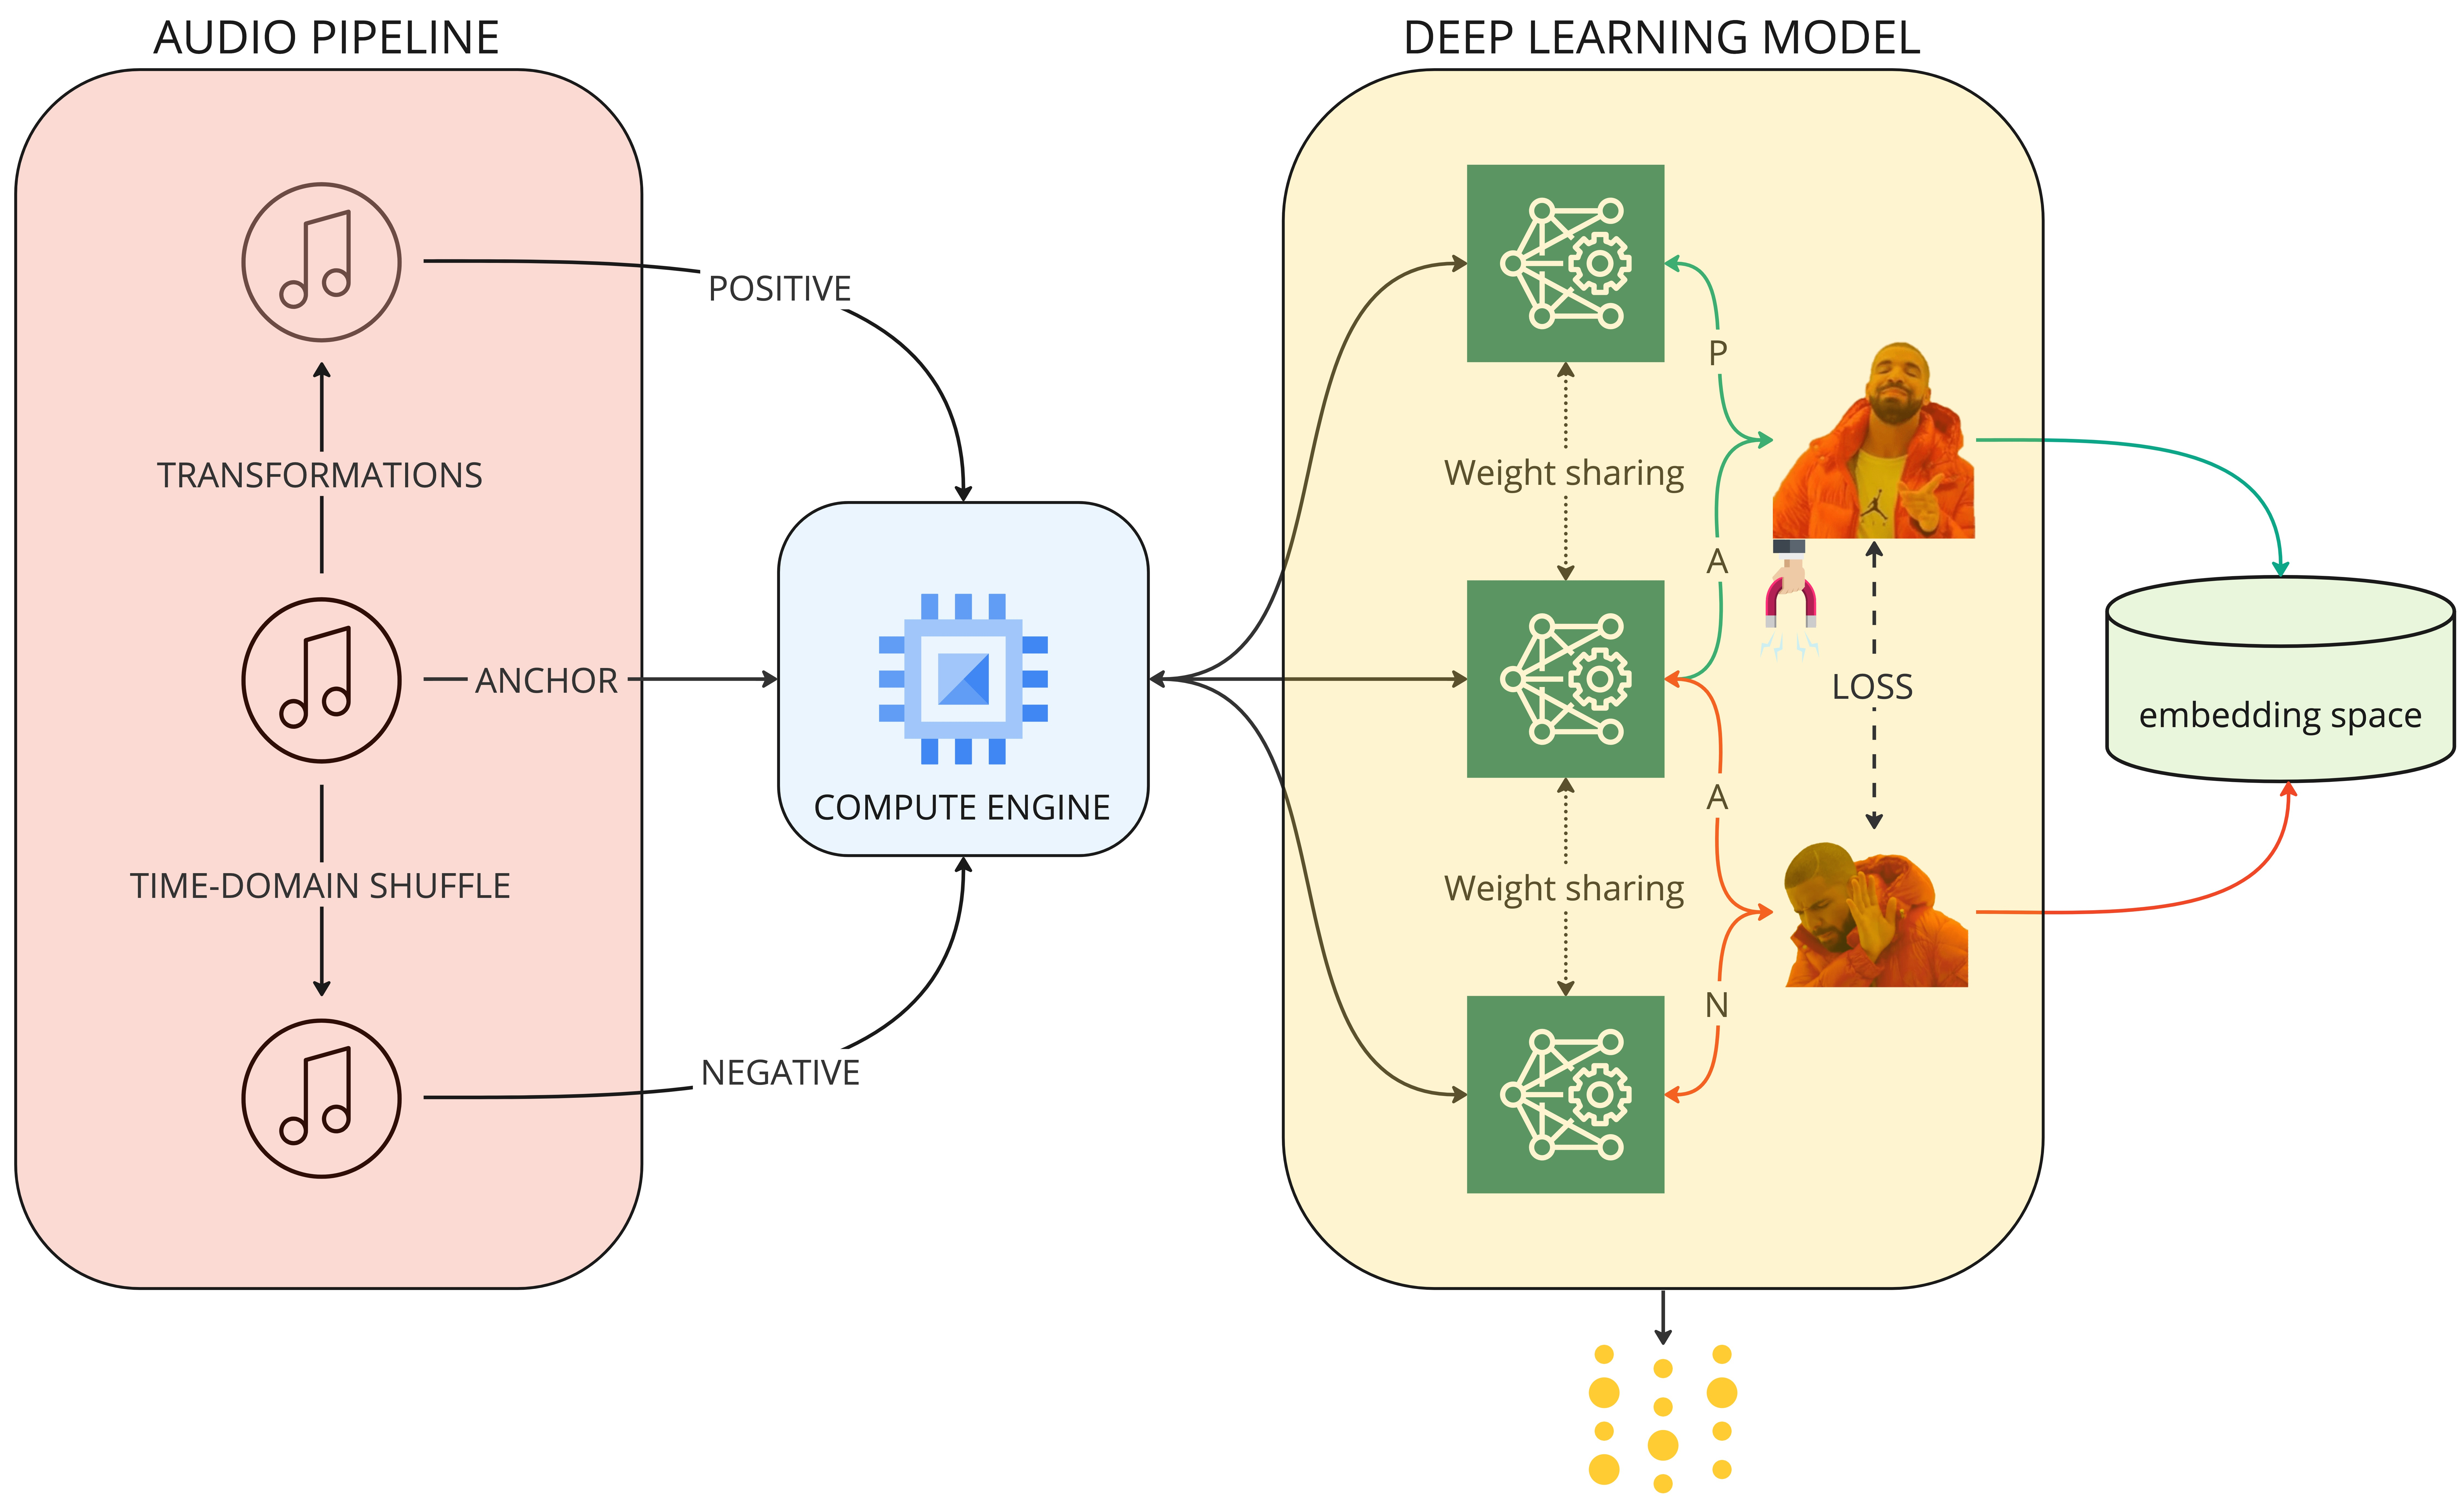
\includegraphics[clip,width=\columnwidth]{figures/images/Triplet Network.jpeg}
    \caption[]{Caption}
    \label{fig:my_label}
\end{figure}



%%%%%BATCH NORM%%%%%%%%%%

In implementing batch normalization, it is necessary to standardize the audio lengths across all elements in the minibatch. We opted to zero-pad all clips to the length of the longest clip, valuing data integrity and completeness over potential performance trade-offs. Thus, the length of the longest array in the batch, which sets the standard for all others, is as follows:

\begin{equation}
L_{\text{max}} = \max_{\text{item} \in \text{batch}}(\max(\text{length}(A_{\text{item}}), \text{length}(P_{\text{item}}), \text{length}(N_{\text{item}})))
\end{equation}
\newpage